\begin{definition}\label{def:trayectoria} {\textbf{Trayectoria.}}
  Se llaman \emph{trayectorias} a las funciones continuas de la forma \[ \boldsymbol{\sigma}:A\subseteq\mathbb{R}\rightarrow B\subseteq\mathbb{R}^m , \quad \text{con } m > 1 .\]    
\end{definition}

\begin{definition}{\textbf{Derivada de una trayectoria.}} 
\label{def:derivada_trayectoria}
Sea $\boldsymbol{\sigma} \colon A \subseteq \mathbb{R} \to \mathbb{R}^m$ una trayectoria definida por sus funciones componentes $$\boldsymbol{\sigma}(t) = (\sigma_1(t), \sigma_2(t), \dots, \sigma_m(t)).$$ Diremos que $\boldsymbol{\sigma}$ es \textit{derivable} en un punto $t_0 \in \interior{A}$ si cada una de sus componentes  es derivable en dicho punto, en dicho caso, se define su derivada evaluada en $t_0$, y se denota por $\boldsymbol{\sigma}'(t_0)$,  a:
\[ 
\boldsymbol{\sigma}'(t_0) = \big(\sigma_1'(t_0), s_2'(t_0), \dots, \sigma_m'(t_0)\big) 
\]
\end{definition}   

 \begin{definition}\label{def:a}
 Una trayectoria $\boldsymbol{\sigma}:[a,b]\subseteq\R\to\Rn{n}$ se la llama de clase $C^1$  si su derivada $\boldsymbol{\sigma}^{\prime}$ existe y es continua en $(a,b)$. 
\end{definition}     
     
\begin{definition}\label{part_intervalos}{\textbf{Partición.}}
Se llama \textit{partición} de un intervalo real $[a,b]$ a un conjunto de puntos 
$P = \{t_0, t_1, t_2, \dots, t_{n-1}, t_n\}$, tal que 
\begin{equation*} 
a = t_0 < t_1 < t_2 < \dots < t_{n-1} < t_n = b. 
\end{equation*} 
Así, la partición $P$ divide al intervalo $[a,b]$ en $n$ subintervalos cerrados de la forma 
\begin{equation*} 
[t_0, t_1], [t_1, t_2], \dots, [t_{n-1}, t_n]. 
\end{equation*} 
\end{definition}



 \begin{definition}\label{def:a-trozos}
 Una trayectoria $\boldsymbol{\sigma}:[a,b]\subseteq\R\to\Rn{n}$ se la llama de clase $C^1$ \emph{a trozos} si existe un conjunto $\{t_i\}_{i=0}^n$ partici\'on de $[a,b]$  (\ref{part_intervalos}) tal que $\boldsymbol{\sigma}$ es de clase $C^{1}$ en $I_i=(t_i, t_{i+1})$ para todo $\:1\leq i \leq n$.
\end{definition}
   

\begin{example}\label{ej:param_circ}  Hallar una trayectoria cuya imagen sea el conjunto $C$ dado por
      \label{ej.: Parametrización circunferencia}
      \begin{equation*}
    C = \{  (x,y)  \in \mathbb{R}^2 \:|\:   x^2+y^2=1 \}.
    \end{equation*}  
\end{example}


\textbf{Soluci\'on. }Recordemos que si punto $(x,y) \in C$  entonces su coordenada $x$  es el coseno del ángulo que forma el eje horizontal con el segmento de radio
que une el origen con tal punto, adem\'as, el seno del ángulo representa la coordenada $y$, tal como se muestra en la Figura \ref{fig:unitCircle1.1}.  
\begin{figure}[H] 
            \centering
            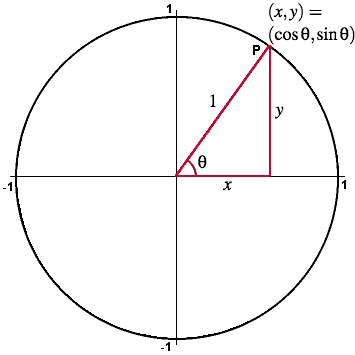
\includegraphics[width=0.5\textwidth]{figs/unitCircle1.png} % Cambia esta ruta por la ubicación de tu imagen
            \caption{Coordenadas de los puntos sobre una circunferencia unitaria.}
            \label{fig:unitCircle1.1} 
\end{figure}
Por lo tanto,  
        \begin{equation}\label{tray1}
            \boldsymbol{\sigma}:[0,2\pi]\rightarrow\mathbb{R}^2\;|\;\boldsymbol{\sigma}(t)=(\cos{t},\sin{t}).
        \end{equation}
cumple lo pedido.       
  
  
\begin{tarea}\label{obs1} Probar que las siguientes  trayectorias   tambi\'en  son solución del Ejemplo \ref{ej:param_circ}, 
\begin{align*}
 \boldsymbol{\sigma}_{1}:[0,2\pi]\rightarrow\mathbb{R}^2\;|\;\boldsymbol{\sigma}_{1}(t)&=(\sin{t},\cos{t} ) \\     
\boldsymbol{\sigma}_{2}:[0,4\pi]\rightarrow\mathbb{R}^2\;|\;\boldsymbol{\sigma}_{2}(t)&= (\cos{t}, \sin{t} ).
\end{align*}   ¿Cu\'antas  soluciones distintas existen ? 
 \end{tarea}       
  
\begin{example}\label{ej:param_circ_1}  Hallar una trayectoria cuya imagen sea el conjunto $C$ dado por
\begin{equation}  
    C = \{  (x,y)  \in \mathbb{R}^2 \:|\:   (x-x_0)^2+(y-y_0)^2=r^2 \} \label{ej}
\end{equation} 
\end{example}

\textbf{Soluci\'on. } Ahora la circunsferencia es de radio $r> 0$ y centro $(x_0,y_0)$  (ver \ref{circ}). Para hallar la trayectoria pedida basta con multiplicar por $r$ a cada componente de (\ref{tray1})  y trasladarla al nuevo centro $(x_0,y_0)$.  Por lo tanto,  una posible respuesta al problema es:
\begin{equation*}
            \boldsymbol{\beta}:[0,2\pi] \rightarrow \mathbb{R}^2  \;|\;  \boldsymbol{\beta}(t)=(r\cos{t},r\sin{t}) + (x_0,y_0)
\end{equation*} 
         
 
 \begin{tarea}\label{obs2} Probar que las siguientes  trayectorias   tambi\'en  son solución del Ejemplo \ref{ej:param_circ_1}, 
\begin{align*}
 \boldsymbol{\beta}_{1}:[0,2\pi]\rightarrow\mathbb{R}^2\;|\;\boldsymbol{\beta}_{1}(t)&=(r\sin{t}+x_0,r\cos{t}+y_0 )  \\  
 \boldsymbol{\beta}_{2}:[0,4\pi]\rightarrow\mathbb{R}^2\;|\;\boldsymbol{\beta}_{2}(t)&=(r\cos{t}+x_0, r\sin{t}+y_0 ).
\end{align*}  ¿Cu\'antas  soluciones distintas existen ? 
 \end{tarea}       
     
     

    
    
\begin{definition}{\textbf{Parametrizaci\'on.}}\label{param}  Dado un conjunto $C \in \mathbb{R}^{n}$ diremos  que

\begin{itemize}

\item[a.]  $\boldsymbol{\sigma}: [a,b] \rightarrow\mathbb{R}^n$  es una parametrizaci\'on de $C$ si 
 $\boldsymbol{\sigma}$ es una trayectoria (\ref{def:trayectoria}) \textbf{ inyectiva } en $(a,b)$   cuya imagen es $C$. En este caso decimos que
$C$ es una curva continua y simple.

\item[b.] La parametrizaci\'on  $\boldsymbol{\sigma}$ es suave si  es de clase $C^{1}$   (\ref{def:a}). En este caso decimos que
$C$ es una curva  suave. 

\item[c.] La parametrizaci\'on  $\boldsymbol{\sigma}$ es suave a trozos si  es de clase $C^{1}$ a trozos (\ref{def:a-trozos}). En este caso decimos que
$C$ es una curva  suave a trozos. 

 \item[d.] La parametrización  $\boldsymbol{\sigma}$  es regular si además de ser suave (a trozos), se verifica que
 $\sigma'(t)\neq 0$  en  $(a,b)$.  En este caso decimos que C es una curva regular.
 
\item[e.]  La parametrización  $\boldsymbol{\sigma}$  es regular a trozos  si además de ser suave (a trozos)  $\sigma'(t)\neq 0$  salvo tal vez en finitos puntos de $(a,b)$.  En este caso decimos que C es una curva regular a trozos.
\end{itemize}
\end{definition} 


\begin{definition} Sea $\boldsymbol{\sigma}: [a,b] \rightarrow\mathbb{R}^n$   una parametrizaci\'on de $C$ entonces $\boldsymbol{\sigma}(a)$ y $\boldsymbol{\sigma}(b)$  se llaman puntos extremos de $C$. Si $\boldsymbol{\sigma}(a)= \boldsymbol{\sigma}(b)$ diremos que $C$ es una curva cerrada. 
\end{definition} 

\begin{example} Las siguientes im\'agenes ilustran 3 curvas.  $\C_1$ una curva simple no cerrada,  $C_2$ una curva no simple  y  $C_3$ una curva simple cerrada.   
\end{example}


\begin{center}
    \begin{tikzpicture}
        
        % Real number line on the left
        \draw[semithick,-Stealth] (-2,0) -- (2,0);
        \node[label=below:$a$] at (-1.25,0) {$[$}; 
        \node[label=below:$b$] at (1.25,0) {$]$}; 
    \node[label=right:$\mathbb{R}$] at (2,0) {};
    
    % Curved arrow in the middle
    \draw[semithick,->] (2,1) to[out=45,in=135,looseness=0.8] (8,1);
    \node[label=below:$\boldsymbol{\sigma}_1$] at (5,2) {};
    
    % Plane R^2 on the right
    \begin{scope}[xshift=8cm]
        \draw[semithick] (0,0) .. controls (1,2) and (2,-1) .. (3,1);
        \node at (0,0) [circle,fill,inner sep=1pt] {};
        \node at (3,1) [circle,fill,inner sep=1pt] {};
        \node[below left] at (0,0) {$\boldsymbol{\sigma}_1(a)$};
        \node[above right] at (3,1) {$\boldsymbol{\sigma}_1(b)$};
    \end{scope}

    \node at (5,-1) [align=center, below] {
                $C_1=\text{Im}(\boldsymbol{\sigma_1})$
            };

\end{tikzpicture}
\end{center}






\begin{center}
\begin{tikzpicture}

    % Real number line on the left
    \draw[semithick,-Stealth] (-2,0) -- (2,0);
    \node[label=below:$a$] at (-1.25,0) {$[$}; 
    \node[label=below:$b$] at (1.25,0) {$]$}; 
    \node[label=right:$\mathbb{R}$] at (2,0) {};

    % Curved arrow in the middle
    \draw[semithick,->] (2,1) to[out=45,in=135,looseness=0.8] (8,1);
    \node[label=below:$\boldsymbol{\sigma}_2$] at (5,2) {};
    
    % Plane R^2 on the right
    \begin{scope}[xshift=8cm, yshift=0.4cm]
        \draw[semithick] 
            (0,0) .. controls (4.5,-1) and (-1.5,-2.5) .. (3,1);
            \node at (0,0) [circle,fill,inner sep=1pt] {};
            \node at (3,1) [circle,fill,inner sep=1pt] {};
    \node[below left] at (0,0) {$\boldsymbol{\sigma}_2(a)$};
    \node[above right] at (3,1) {$\boldsymbol{\sigma}_2(b)$};
    \end{scope}

    \node at (5,-1) [align=center, below] {
                $C_2=\text{Im}(\boldsymbol{\sigma_2})$
            };

\end{tikzpicture}
\end{center}






\begin{center}
 \tikzsetnextfilename{curva-cerrada}  
\begin{tikzpicture}
  
    % Real number line on the left
    \draw[semithick,-Stealth] (-2,0) -- (2,0);
    \node[label=below:$a$] at (-1.25,0) {$[$}; 
    \node[label=below:$b$] at (1.25,0) {$]$}; 
    \node[label=right:$\mathbb{R}$] at (2,0) {};
    
    % Curved arrow in the middle
    \draw[semithick,->] (2,1) to[out=45,in=135,looseness=0.8] (8,1);
    \node[label=below:$\boldsymbol{\sigma}_3$] at (5,2) {};
    
    % Plane R^2 on the right
    \begin{scope}[xshift=8.2cm, yshift=0.5cm]
        \draw[semithick]
            plot[smooth,tension=1.2] coordinates {(1,0.6) (3,0) (2.5,-1.5) (1,-1) (0,0) (1,0.6)};
    
            % \foreach \point in {(1,0.6), (3,0), (2.5,-1.5), (1,-1), (0.2,0.1), (1,0.6)} {
            % \node at \point [circle,fill,inner sep=1pt] {};
            % }
        \node at (0,0) [circle,fill,inner sep=1pt] {};
        \node[below left] at (0,0) {$\boldsymbol{\sigma}_3(a)=\boldsymbol{\sigma}_3(b)$};
    \end{scope}

 \node at (5,-1) [align=center, below] {
                $C_3=\text{Im}(\boldsymbol{\sigma_3})$
            };

\end{tikzpicture}
\end{center}



\begin{definition}\label{orien}  \textbf{Orientaci\'on para curvas simples.}   Sea $C$  una curva simple. Se denomina \emph{orientación} de $C$ a la elección de un sentido de recorrido a lo largo de la curva. Cada curva simple admite exactamente dos orientaciones posibles, correspondientes a los dos sentidos opuestos en los que puede ser recorrida.  Sean  $P$ y $Q$  los extremos de la curva. Si  $P\neq Q$,  entonces podemos considerar a $C$ con orientaci\'on desde $P$ hacia $Q$ o bien desde $Q$ hacia $P$.   Si  $P= Q$  (curva cerrada) y  $C \subset \mathbb{R}^{2}$ 
, una orientación se dice  \emph{antihoraria} o \emph{positiva} si  al recorrer la curva según dicha orientación, la región acotada por $C$  queda siempre a la izquierda del sentido de recorrido. En cambio, la orientación opuesta  se denomina \emph{horaria} o \emph{negativa}.  \\ En general a una curva simple $C$ junto con una orientaci\'on la notaremos por $C$ junto a un signo $+$ (o $-$) usado como  supra\'indice, quedando $C^{+}$  (o $C^{-}).$  Por ejemplo, si elegimos notar a una curva simple no cerrada $C$ orientada desde $P$ hacia $Q$  por  $C^{+}$  entonces  $C^{-}$ ser\'a la orientaci\'on inversa ( desde $Q$ hacia $P$).
\end{definition}


\begin{definition} \textbf{Orientación inducida sobre  curvas simples.} Sea \( C \) una curva simple en \( \mathbb{R}^n \) y sea  
$\boldsymbol{\sigma} : [a,b] \to \mathbb{R}^n$ una parametrización regular de \( C \).  Entonces, se dice que la parametrización \( \boldsymbol{\sigma} \)  \emph{induce una orientación sobre la curva \( C \)}. Esta orientación consiste en recorrer la curva desde el punto \( \boldsymbol{\sigma}(a) \) hasta el punto \( \boldsymbol{\sigma}(b) \), siguiendo la dirección del vector tangente \( \boldsymbol{\sigma}'(t) \).
\end{definition} 

\begin{definition}\label{orien_pre}
Sea $C^{+}$ una curva simple orientada (\textit{ i.e} con una orientaci\'on dada) y sea $\boldsymbol{\sigma} : [a,b] \to \mathbb{R}^n$ una parametrización  de \( C \). Diremos que  $\sigma$ \textit{preserva la orientación} de la curva orientada \( C \) si el sentido en que la recorre coincide con la orientación dada.  En caso contrario, diremos que  $\sigma$ \textit{ no preserva} o  \textit{invierte la orientación} de $C$. 
\end{definition} 




\begin{tarea}
Ver cuales de las trayectorias encontradas en (\ref{obs1}) y (\ref{obs2}) son parametrizaciones y, en tal caso,  dar la orientraciones inducidas por ellas sobre las curvas.  
\end{tarea}
    
    
    
    
% \begin{obs}    Otra forma clásica de parametrizar el conjunto $C$ dado en (\ref{ej})  es posicionarse en el punto $(x_0-r,y_0)\in C$ y
 %       luego, desde ese punto,  graficar rectas de pendientes variables. Cada una de esas rectas interseca con $C$ en exactamente dos puntos,
 %       siendo uno de ellos el punto inicial.  Así, si se grafican rectas con todas las pendientes posibles, se intersecará C en todos sus puntos.
 %           \begin{figure}[H]
 %     \begin{center}
 %     \begin{tikzpicture}[scale=3]
 %         % Parámetros
 %         \def\xo{1}    % centro x
 %         \def\yo{1}    % centro y
 %         \def\r{1}     % radio

          % Punto fijo de la parametrización (en el borde izquierdo de la circunferencia)
 %         \coordinate (F) at ({\xo - \r}, {\yo});
          
 %         % Dibuja la circunferencia
 %%         \draw[thick,blue!40] (\xo,\yo) circle(\r);
 %         \node[below left,red] at (F) {$(x_0 - r,\ y_0)$};

          % Dibuja el centro
 %         \filldraw[black] (\xo,\yo) circle(0.015) node[below right] {$(x_0,y_0)$};

          % Dibuja el punto fijo
 %         \filldraw[red] (F) circle(0.015);

          % Dibuja algunos puntos sobre la circunferencia usando la parametrización racional
 %         \foreach \t in {-2, -0.5, 0.5, 1.5, 4} {
              % Coordenadas parametrizadas
 %             \pgfmathsetmacro{\xr}{\r*(1 - (\t)^2)/(1 + (\t)^2) + \xo}
 %             \pgfmathsetmacro{\yr}{\r*(2*\t)/(1 + (\t)^2) + \yo}
 %             \coordinate (P) at (\xr,\yr);

              % Dibuja el punto generado
 %             \filldraw[black] (P) circle(0.015);
              % Dibuja la recta desde el punto fijo al punto generado
 %             \draw[dashed,gray] (F) -- (P);
 %         }

 %     \end{tikzpicture}
 %     \caption{Representación de una forma alternativa de parametrizar la circunferencia.}
 %     \end{center}
 % \end{figure}
 % Para ello, elegimos los puntos $(x,y)$ pertenecientes a la imagen de la parametrización alternativa $\boldsymbol{\sigma}^*(t)$ como la intersección de
 %       \begin{equation*}
 %         (x-x_0)^2+(y-y_0)^2=r^2 \quad\land\quad y=t(x-(x_0-r))+y_0,\quad \forall t\in \mathbb{R}.
 %       \end{equation*}
 %       Resolviendo ese sistema de ecuaciones para cada $t$, para encontrar la solución distinta a $(x_0-r,y_0)$ resulta que
 %       \begin{equation*}
 %         \boldsymbol{\sigma}^*:\mathbb{R}\rightarrow\mathbb{R}^2\;|\; \\ \boldsymbol{\sigma}^*(t)=\left(r\frac{1-t^2}{1+t^2}+x_0,r\frac{2t}{1+t^2}+y_0\right).
 %%       \end{equation*}
 %   \end{obs}
